% DRAFT 2 — MINIMALIST (poster2.tex). Build: pdflatex poster2.tex (twice)
\documentclass[final]{beamer}
\usepackage[orientation=portrait, size=a0, scale=0.98]{beamerposter}
\usepackage[T1]{fontenc}
\usepackage[utf8]{inputenc}
\usepackage[scaled=0.92]{helvet}
\renewcommand{\familydefault}{\sfdefault}
\usepackage{lmodern}
\usepackage{amsmath,amssymb}
\usepackage{booktabs}
\usepackage{graphicx}
\usepackage{ragged2e}
\usepackage{xcolor}
\usepackage{tikz}
\usetikzlibrary{shapes,shadows,arrows.meta,positioning,calc}
\usepackage{pgfplots}
\pgfplotsset{compat=1.18}
\setlength{\overfullrule}{4pt}
\definecolor{navy}{HTML}{0E2A47}
\definecolor{navy2}{HTML}{14456E}
\definecolor{accent}{HTML}{0091B3}
\definecolor{accent2}{HTML}{E27A1E}
\definecolor{panel}{HTML}{F2F6FA}
\definecolor{panel2}{HTML}{E4EDF6}
\definecolor{good}{HTML}{1E7B4F}
\definecolor{bad}{HTML}{B13325}
\definecolor{gold}{HTML}{C79A2B}
\setbeamercolor{block title}{fg=white, bg=navy}
\setbeamercolor{block body}{fg=black!88, bg=panel}
\setbeamerfont{block title}{size=\Large, series=\bfseries}
\setbeamerfont{block body}{size=\Large}
\setbeamercolor{itemize item}{fg=accent}
\setbeamertemplate{itemize item}{\raisebox{0.35ex}{\small$\blacktriangleright$}}
\setlength{\leftmargini}{1.1cm}
\setbeamertemplate{itemize/enumerate body begin}{\setlength{\itemsep}{0.25cm}}
\newlength{\blocklskip}\setlength{\blocklskip}{0.55cm}
\newlength{\blockrskip}\setlength{\blockrskip}{0.55cm}
\setbeamertemplate{block begin}{%
  \par\vskip0.55cm%
  \begin{beamercolorbox}[wd=\linewidth,leftskip=0.5cm,rightskip=0.5cm,sep=0.25cm]{block title}%
    \usebeamerfont*{block title}\insertblocktitle%
  \end{beamercolorbox}%
  {\nointerlineskip\vskip-0.5pt}%
  \usebeamerfont{block body}%
  \begin{beamercolorbox}[wd=\linewidth,leftskip=\blocklskip,rightskip=\blockrskip,vmode]{block body}%
    \setlength{\linewidth}{\dimexpr\linewidth-\blocklskip-\blockrskip\relax}%
    \setlength{\hsize}{\linewidth}\setlength{\textwidth}{\linewidth}\setlength{\columnwidth}{\linewidth}%
    \setlength{\parskip}{0.28cm}\justifying%
}
\setbeamertemplate{block end}{\end{beamercolorbox}\vspace*{0.15cm}}
\setbeamertemplate{navigation symbols}{}
\setbeamertemplate{headline}{}
\setbeamertemplate{footline}{}
\setbeamersize{text margin left=1.0cm, text margin right=1.0cm}
\newcommand{\hl}[1]{\textbf{\textcolor{navy2}{#1}}}
\newcommand{\code}[1]{{\ttfamily\small #1}}
\newcommand{\figcap}[1]{{\centering\small\itshape\color{black!62} #1\par}}
\newcommand{\kpi}[3]{%
  \begin{minipage}[t]{0.235\linewidth}\centering
    {\color{#3}\fontsize{30}{30}\selectfont\bfseries #1}\\[0.08cm]
    {\small\bfseries #2}%
  \end{minipage}%
}
\tikzset{
  laybox/.style={rounded corners=14pt, draw=navy, line width=2.5pt, fill=white,
    minimum width=13.2cm, minimum height=15.5cm, align=center, text width=12.4cm,
    drop shadow={shadow xshift=3pt, shadow yshift=-3pt, opacity=0.18}},
  laytitle/.style={fill=navy, text=white, font=\bfseries\Large, rounded corners=8pt,
    minimum width=11.2cm, minimum height=1.6cm, align=center, text width=10.8cm},
  arrowbig/.style={{Stealth[length=14pt,width=10pt]}-, line width=4pt, draw=accent},
  arrowthin/.style={{Stealth[length=11pt,width=8pt]}-, line width=3pt, draw=good},
}
\begin{document}
\begin{frame}[t]
\begin{beamercolorbox}[wd=\textwidth,leftskip=1.2cm,rightskip=1.2cm,sep=0.55cm]{block title}
\centering
{\fontsize{44}{46}\selectfont\bfseries Fusing LLM Semantic Repair with Genetic Programming for Robust Alpha Discovery\par}
\vspace{0.25cm}
{\Large G.S.K. Raghav Anand \textbullet\ NIT India \textbullet\ IEEE Access manuscript\par}
\vspace{0.2cm}
{\large\itshape Vanilla quant models break out-of-sample. A regime-aware GP + local-LLM repair loop fixes that --- S\&P 500 Sharpe decay cut from \textbf{$-35\%$ to $-7\%$}.}
\end{beamercolorbox}
\vskip0.3cm
\begin{beamercolorbox}[wd=\textwidth,leftskip=0.8cm,rightskip=0.8cm,sep=0.35cm]{block body}
\centering
\kpi{10.6\%}{net return (peak)}{good}\hfill
\kpi{0.65}{net Sharpe}{navy2}\hfill
\kpi{$-7\%$}{S\&P decay (was $-35\%$)}{good}\hfill
\kpi{+18\%}{over quant ceiling}{accent2}\\[0.1cm]
{\small NSE Nifty 50 2002--2025 (23 yrs) \textbullet\ validated on S\&P 500 + SSE \textbullet\ costs 20+10 bps, cap INR 50 Cr \textbullet\ local Llama-3.2-3B + Gemma-2-2B, \$0 inference}
\end{beamercolorbox}
\vskip0.2cm
\begin{block}{SYSTEM ARCHITECTURE --- read left to right (the core of this poster)}
\centering
\begin{tikzpicture}[node distance=0.6cm, font=\small]
\node[laybox, fill=gold!14] (data) {
  \tikz{\node[laytitle, fill=gold!85!black] {0 DATA};}
  \\[0.15cm]{\Large\bfseries NSE 50}\\[-0.05cm]{\normalsize 2002--2025 daily OHLCV}
  \\[0.08cm]{\normalsize + PE / ROE / EPS / BV}\\[0.08cm]{\normalsize S\&P 500 + SSE for test}
  \\[0.12cm]{\Large\bfseries\color{gold!70!black} What goes in}
};
\node[laybox, right=0.7cm of data] (afm) {
  \tikz{\node[laytitle] {1 AFM (slow)};}
  \\[0.15cm]{\Large\bfseries Macro anchor}\\[-0.05cm]{\normalsize FinBERT sentiment}
  \\[-0.05cm]{\normalsize + fundamentals}
  \\[0.12cm]{\Large\bfseries\color{navy2} Bull / bear prior}
  \\[-0.05cm]{\normalsize stops GP chasing noise}
};
\node[laybox, right=0.7cm of afm] (hmm) {
  \tikz{\node[laytitle] {2 HMM (fast)};}
  \\[0.15cm]{\Large\bfseries 2 volatility states}\\[-0.05cm]{\normalsize calm vs turbulent}
  \\[-0.05cm]{\normalsize Baum-Welch + Viterbi}
  \\[0.12cm]{\Large\bfseries\color{navy2} Which regime now?}
  \\[-0.05cm]{\normalsize routes to specialist}
};
\node[laybox, right=0.7cm of hmm] (gp) {
  \tikz{\node[laytitle, fill=accent!85!black] {3 GP SEARCH};}
  \\[0.15cm]{\Large\bfseries Evolves formulas}\\[-0.05cm]{\normalsize pop 500, depth max 6}
  \\[-0.05cm]{\normalsize Sharpe minus bloat fitness}
  \\[0.12cm]{\Large\bfseries\color{accent!80!black} Invents alphas}
};
\node[laybox, right=0.7cm of gp, draw=good, line width=3.5pt] (llm) {
  \tikz{\node[laytitle, fill=good] {4 LLM REPAIR};}
  \\[0.15cm]{\Large\bfseries Judge, then fix}\\[-0.05cm]{\normalsize Llama scores 1--5}
  \\[-0.05cm]{\normalsize Gemma rewrites S below 3}
  \\[0.12cm]{\Large\bfseries\color{good} Repair, not reject}
};
\draw[arrowbig] (data.east) -- (afm.west);
\draw[arrowbig] (afm.east) -- (hmm.west);
\draw[arrowbig] (hmm.east) -- (gp.west);
\draw[arrowbig] (gp.east) -- (llm.west);
\node[below=0.9cm of gp, font=\Large\bfseries, color=good] (loop)
  {repaired tree recompiled, back into evolution (zero attrition)};
\draw[arrowthin] (llm.south) |- (loop.east);
\draw[arrowthin] (loop.west) -| (gp.south);
\node[below=1.9cm of loop, rounded corners=12pt, fill=navy, text=white,
  minimum width=60cm, minimum height=2.4cm, align=center, font=\Large]
  (out) {\textbf{OUTPUT:} regime alphas x (AFM prior + HMM state) = dollar-neutral top/bottom-15\% portfolio, monthly rebalance};
\end{tikzpicture}
\figcap{Follow the five boxes once and you understand the paper. Green loop is the novelty: old hybrids deleted bad trees; this repairs them.}
\end{block}
\begin{columns}[t,onlytextwidth]
\column{0.325\linewidth}
\begin{block}{1 Problem in 30 seconds}
\begin{itemize}
  \item Quant factors \hl{decay}: top-1000 anomalies lose about 32\% after publication; GP memorises noise.
  \item Old LLM+GP hybrids \hl{delete} bad formulas and lose diversity.
  \item Fix: \hl{repair, don't reject} --- rewrite only the truly nonsensical (score 2 or less).
\end{itemize}
\end{block}
\begin{block}{2 What each layer does}
\begin{itemize}
  \item \hl{AFM (slow):} news mood + PE/ROE/EPS/BV gives a bull/bear prior, an economic compass.
  \item \hl{HMM (fast):} 2-state volatility filter. Calm goes to trend formulas; turbulence to reversals + quality.
  \item \hl{GP (inventor):} 500 trees, depth max 6, Sharpe minus complexity fitness.
  \item \hl{LLM (editor):} Llama rates economics 1--5; Gemma rewrites failures from a closed vocabulary.
  \item \hl{Settings:} AFM FinBERT threshold $\tau=0.5$; HMM 2-state Baum--Welch + Viterbi; GP pop 500, depth max 6; edit list $L\le5$; dollar-neutral top/bottom-15\%, monthly rebalance.
\end{itemize}
\end{block}
\begin{block}{2b Loop + stability (how it runs, why it holds)}
GP loop: AFM prior + HMM state $\to$ fitness (Sharpe $-$ complexity) $\to$ Llama judge (1--5) $\to$ Gemma repair ($S\le2$, closed vocab, $L\le5$) $\to$ recompile, back into evolution. Zero attrition: every repair compiles.
\centering
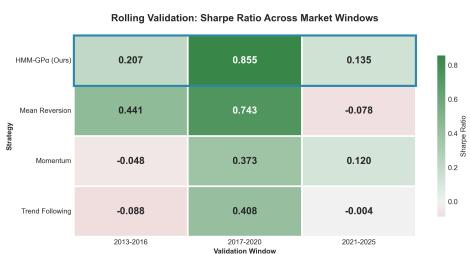
\includegraphics[width=0.92\linewidth,keepaspectratio]{images/28656a9cc9f26a4ffd2ce0ab7611324d8cd0fff6192ee9abf348a58dd50cc0a7.jpg}
\figcap{Rolling-window Sharpe stays positive (0.855) in turbulent 2017--20 where momentum + trend turn negative. Regime specialists, not one average model.}
\end{block}
\column{0.345\linewidth}
\begin{block}{3 Does it work? Each layer adds return (NSE)}
\centering

\includegraphics[width=\linewidth,keepaspectratio]{images/5c0699b6596fbda008d867190a140e7a93dde191b609f3beaa28ce350f2f58d2.jpg}
\figcap{Ablation, NSE net: Vanilla 1.62\% $\to$ +AFM 6.43\% $\to$ +HMM 8.41\% $\to$ +LLM 9.61\%. AFM anchors context; HMM specialises; LLM repair beats the quant ceiling.}
\end{block}
\begin{block}{4 Decay: S\&P halved, SSE quartered (Sharpe change)}
\centering
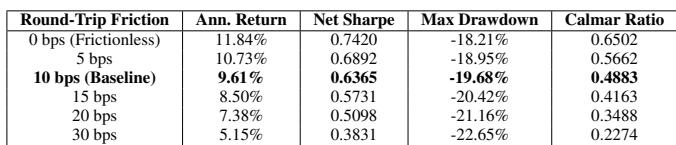
\includegraphics[width=\linewidth,keepaspectratio]{images/59097310a5a6569dcd4fcfb5fd1b63f2db1743a708a472db6705d78f730e458b.jpg}
\figcap{S\&P decay -35.03\% to -6.77\%. China -92.08\% to -46.68\%. Repair removes overfit noise instead of deleting trees.}
\end{block}
\column{0.325\linewidth}
\begin{block}{5 What the machine rediscovers (feature mix)}
\centering
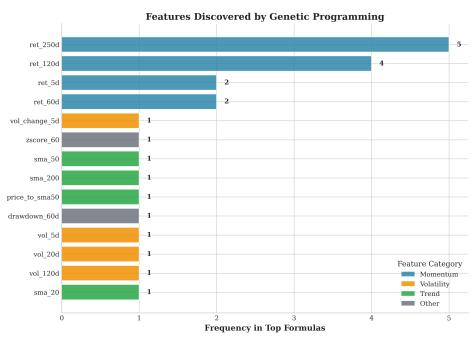
\includegraphics[width=0.92\linewidth,keepaspectratio]{images/97b82991ea2743e616388671ed37ff6bea3cc310277e70b8b60047cb29f427af.jpg}
\figcap{Feature mix of top alphas (paper Fig.~6): intermediate momentum + volatility scalers dominate. Sensible economics: trends in calm markets, reversals + quality in stress.}
\end{block}
\begin{block}{6 Read this and leave (5-min summary)}
\begin{itemize}
  \item \hl{Robust every year:} positive Sharpe 2019--25 incl.\ COVID (-14.8\% DD vs -38.5\% momentum).
  \item \hl{Deployable:} about \$250M capacity; costs in; \$0 inference (local 3B/2B models).
  \item \hl{Next:} NSE 500, LoRA-Gemma, multi-agent judges.
\end{itemize}
\begin{beamercolorbox}[wd=\linewidth,leftskip=0.35cm,rightskip=0.35cm,sep=0.3cm]{block title}
\centering\Large\bfseries Take-away: semantic repair is a free regulariser, India to US to China.
\end{beamercolorbox}
\end{block}
\begin{block}{7 Repair example + wealth curve + regimes (one glance)}
Before (1/5): \code{add(log(vol\_5d), sin(p\_to\_sma20))} --- sine on prices is noise. After (4/5): \code{div(ret\_20d, ts\_mean(vol\_20d,20))} --- risk-adjusted momentum. Rank IC $-0.012 \to +0.038$; 100\% repairs compile, zero crashes over 1,729 days.\\[0.15cm]
\noindent\begin{minipage}[t]{0.49\linewidth}\centering
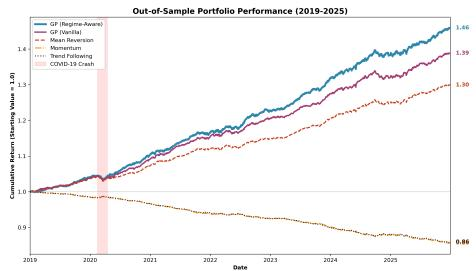
\includegraphics[width=\linewidth,keepaspectratio]{images/ed7d3491c0ec3faa565111046b72b92898718e516bf5ea024476263ee826a05c.jpg}
\\{\small\itshape Wealth 2019--25 compounds through bull + bear (momentum DD $-40.65\%$).\par}
\end{minipage}\hfill
\begin{minipage}[t]{0.49\linewidth}\centering
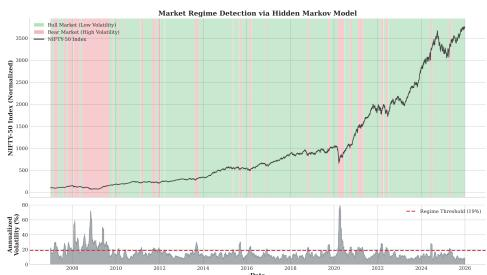
\includegraphics[width=\linewidth,keepaspectratio]{images/33f0cbdd4e18c1897be25763a9a2422f0e044cbf536822f96ca1ea48c66eb838.jpg}
\\{\small\itshape HMM: State 0 calm expansion vs State 1 turbulence (COVID-2020, tightening-2022); stickiness 0.994/0.983.\par}
\end{minipage}
\figcap{Repair turns nonsense into economics; regime routing is why wealth survives shocks.}
\end{block}
\end{columns}
\vskip0.25cm
\begin{beamercolorbox}[wd=\textwidth,sep=0.3cm]{block body}
{\small\raggedright
\textbf{Refs:} Kakushadze 101 Alphas (2016) \textbullet\ AlphaAgent arXiv:2502.16789 \textbullet\ TEDE (2026) \textbullet\ DEAP JMLR \textbullet\ Hamilton (1989) McLean (2016) \textbullet\ Almgren--Chriss (2000).
NSE 50 2002--25; S\&P 500 + SSE transfer test. Draft 1 (poster.pdf) kept as full version.
}
\end{beamercolorbox}
\end{frame}
\end{document}
